\subsection{Introduction to Dynamic Systems and Control}
\label{chapter:dynamic_systems_and_control}

The purpose of this section is to present the field of dynamic systems and control to a reader who
is not familiar with the topic. Our goal is to demonstrate the huge technological significance of
control system design, and to make clear that the methods used in this paper are all very much
standard practice. Other than the original insight of the application of control system design to
the economic problem, the analysis is nothing new, albeit presented in a somewhat unusual way so as
to provide a crash-course in the intuitions and basic analytical method while avoiding formal
mathematical methods.

\subsection{Huygens, Watt, Maxwell and the Wright Brothers}

TODO: Huygens

TODO: Watt

TODO: Maxwell

Prior to the Wright brother's first flight in December 1903, Orville and Wilbur Wright believed that
the most fundamental problems they needed to solve were control problems. In September 1901 Wilbur
Wright's first public presentation on the feasibility of heavier-than-air flight stated that ``When
this one feature [control] has been worked out the age of flying machines will have arrived, for all
other difficulties are of minor importance."\cite{wright1908}


% We are looking for a way that we can keep the conditions of the system in some desirable state.
% Examples are ... If the system is predictable can use an open system. Many systems, however are not
% completely predictable. In many case, despite the unpredictability we can still control the system
% to a certain degree. One method is to use a closed system. Another method is to introduce a
% sophisticated controller into the loop, such as a human, in combination with the mechanism. Examples
% are ...
% 
% A heater with a fixed output.
% 
% A heater with a thermostat.
% 
% Using a schema similar to \ref{fig:feedback_schema} we can represent the cyclist as,
% 
% \begin{figure}[H]
% \centering
% 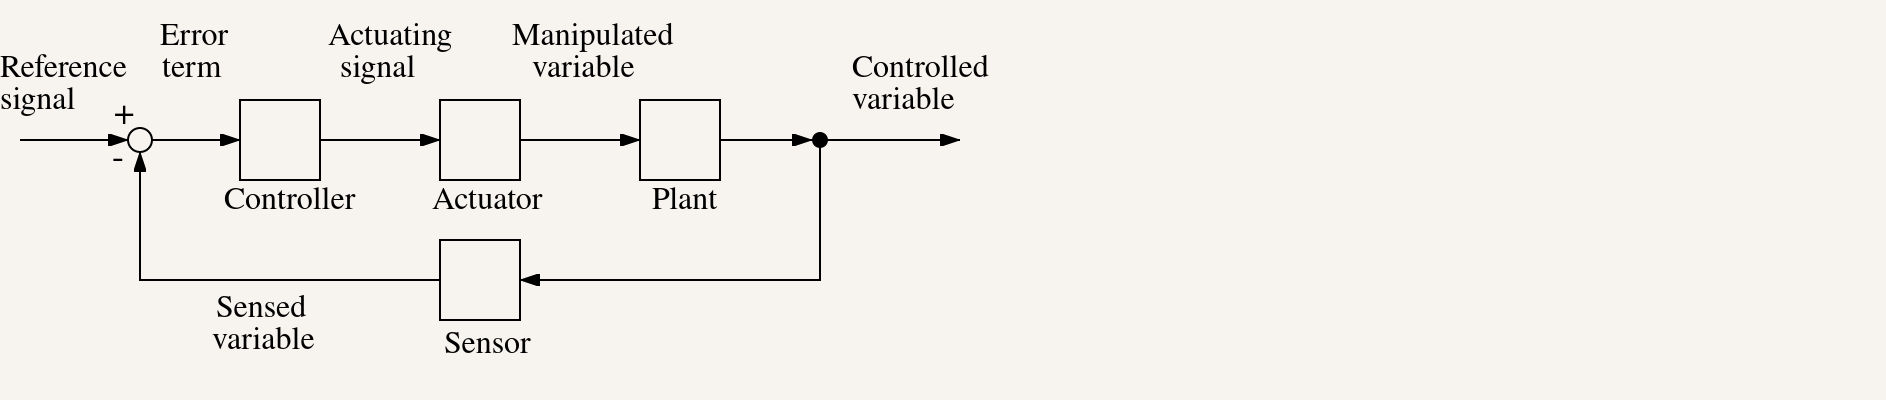
\includegraphics[scale=0.48]{02_dynamic_systems_and_control/png/bicycle_feedback_schema}
% \caption{Bicycle Feedback Schema}
% \label{fig:bicycle_feedback_schema}
% \end{figure}
% 
% The 'reference signal' or 'set point' is the goal of the system, in this case most likely a
% desination and when they want to arrive. The controller takes the set point and the present
% conditions, i.e. where the cyclist is currently, the location of obstacles, if the road is heading
% uphill or downhill etc.  weather conditions are, how much time they have remaining and convert this
% into a control signal. Part of the control signal in this case is observable - the person's
% adjustments to the handle-bars, other signals are not observable such as decisions on how hard to
% pedal. The actuator in this case is the cyclists leg muscles, which convert those desicions, and use
% energy to convert them into pedal pressure. The cyclist then observes the situation again and reacts
% to the situation by feeding their sensory data back into the 'controller' and so on in a closed
% loop. In the case of the cyclist we depend on continuous inputs in a changing, often unpredictable
% environment to adjust behaviour - we require a closed loop system.
% 
% \subsubsection{Huygens}
% 
% \subsubsection{Watt}
% 
% \subsection{PID controller}
% 
% \subsubsection{James Clerk Maxwell}
% 
% \subsubsection{The Wright Brothers}
% 
% Prior to the Wright brother's first flight in December 1903, Orville and Wilbur Wright believed that
% the most fundamental problems they needed to solve were control problems. In September 1901 Wilbur
% Wright's first public presentation on the feasibility of heavier-than-air flight stated that ``When
% this one feature [control] has been worked out the age of flying machines will have arrived, for all
% other difficulties are of minor importance."\cite{wright1908}
% 
% % TODO - this paragraph requires work.
% 
% The general view prior to the Wright brothers was that aircraft required the mechanism to
% self-stabilize. [this was a problem because incorporating stability into the air-craft was at the
% cost of agility. Possibly because the Wright brothers were bicycle-shop owners, and were aware that
% bicycles are fundamentally unstable and require human intervention to stay upright, they understood
% that this control could be done by the pilot rather than the plane.
% 
% \subsubsection{Elmer Sperry}
% 
% Elmer Sperry was the first to construct a PID controller. One notable characteristic of PID
% controllers is that despite much work in the design of more sophisticated controllers, PID
% controllers are by far the most widely used, demonstrating robustness to solve a broad range of
% control problems.
% 
% Elmer Sperry is best known for his construction and application of gyroscopes following the
% invention of the first practical gyroscope by Hermann Anschütz-Kaempfe in 1904. One of Sperry's
% applications was the use of a gyroscope as a component in a control system to self-stabilize
% airplanes.
% 
% [longer flights]
%  
% Following on from these experiences, he worked with the U.S. Navy to use gyroscopes for stabilizing
% ships, and then also to build control systems as auto-pilots of ships. Because the control process
% involved in steering large ships with significant lags and so was relative slow and visible, he was
% able to observe that skilled helmsmen used a more nuanced 'algorithm' than just a proportional
% response, and that the helmsman with put the helm over in the opposite to the directions in which
% the ship was yawing a significantly in advance (a D response), and that helmsman worked the ship
% upwards in response to currents and prevailing wind (an I response). Sperry then incorporated these
% three responses (P, I and D) into his mechanical control mechanism which connected the gyroscope to
% the ships steering.
% 
% In 1922 Nicolas Minorsky published a paper which encapsulated the P, I and D into an
% equation.\cite{minorsky1922}
% 
% % chapter:          Dynamic Systems
% % section:          Positive Feedback
% \section{Positive Feedback}
% 
% % chapter:          Dynamic Systems
% % section:          Error Correction
% \section{Error Correction}
% 
% % chapter:          Dynamic Systems
% % section:          Isolation 
% \section{Isolation}
% 
% % chapter:          Dynamic Systems
% % section:          Stability
% \section{Stability}
% 
% % chapter:          Dynamic Systems
% % section:          Internet
% \section{Internet}
% 
% % chapter:          Dynamic Systems
% % section:          Internet
% % subsection:       The Network 
% \subsection{The Network}
% 
% The most notable difference between digital networks and the precursor to digital networks - the
% telephone network - was the notion of packet switching.
% 
% % Baran
% 
% In the mid 1960s Paul Baran was working on the problem of fault-tolerant networks\cite{baran1964intro}.
% 
% \begin{quote}
% Packet switching technology was not really an invention, but a reapplication of the basic
%     dynamic-allocation techniques used for over a century by the mail, telegraph, and torn paper
%     tape switching systems. \cite{roberts1978}
% \end{quote}
% 
% % Pre-allocation
% 
% radio, telephony
% 
% Analog telephone systems work by setting up a connection between two telephones. This connection
% takes complete ownership of the physical connection, the wire. Baran proposed to share the physical
% wire between many connections. Time division multiplexing had been used since the late 19th century
% to share a single wire to send multiple telegraph messages synchronously. This was called time
% division multiplexing. The idea was to share the wire by allocating divisions of time for each
% message. Baran's idea was rather than to multiplex by time, to multiplex by a standardized message
% block, later termed a 'packet'.
% 
% % Dynamic allocation
% 
% telegraph and mail systems
% 
% \begin{quote}
% Time division multiplexing appears so natural to data transmission that we might wish to consider an
% alternative approach -- a standardized message block as a network interface standard.\cite{baran1964intro}
% \end{quote}
% 
% The reasons were
% 
% % Efficiency
% 
% telephone systems multiplex, i.e. chop up and share out communication by pre-allocating transmission
% bandwidth a connect (or telephone call). Data transmission comes in short bursts, so the complete
% physical connection is 'blocked' by the empty parts in a transmission, and so roughly 90 percent of
% capacity was wasted. We can see why telegraphy was so much cheaper than voice communication. By
% reducing the granularity of the chopping-up into small packets, one could more efficiently share out
% the resource, by filling up the blank spaces by some other communication.
% 
% % Reliability
% 
% % Dynamics
% 
% A telephone call fixes the relationship between transmitted information and the network. By
% packaging up information and assigning each package a destination address, a degree of freedom is
% introduced between the transmitted information and the network. This means that information can be
% rerouted, i.e. respond to network conditions, directly attacking the problem of network fault
% tolerance. We have introduced a negative feedback here, i.e. a response to failure in the network,
% so as to maintain a stable condition i.e. the success rate of transmissions. We'll look at how this
% is implemented in section A.
% 
% Such dynamic systems require feedback for regulation.
% 
% % chapter:          Dynamic Systems
% % section:          Internet
% % subsection:       Introduction
% % subsubsection:    Some Abstractions - Hiding 
% \subsubsection{Some Abstractions - Hiding}
% 
% % TODO: Need a 'hindsight' qualification.
% 
% % chapter:          Dynamic Systems
% % section:          Internet
% % subsection:       Introduction
% % subsubsection:    Some Constraints - Distributed Systems 
% \subsubsection{Some Constraints - Distributed Systems}
% 
% \subsubsection{Some Constraints - Burstiness}
% 
% \subsubsection{Some Constraints - Heterogenous Networks and Hardware}
% 
% In the early 1970s a protocol for joining together many networks. The question is why would you
% join together networks, each with their own hardware and protocols? Why not select a uniform
% protocol that is universal across all networks?
% 
% \begin{quote}
%     Even though many different and complex problems must be solved in the design of an individual
%     packet switching network, these problems are manifestly compounded when dissimilar networks are
%     interconnected. Issues arise which may have no direct counterpart in an individual network and
%     which strongly influence the way in which internetwork communication can take place.
%     \cite{cerf1974}
% \end{quote}
% 
% % TODO: Answer this question
% 
% % This section should probably be shifted to a later section.
% 
% The main problem of building a network of networks, i.e. the internet was to figure out a way for
% many different kinds of networks to interoperate. In the foundational paper outlining how to
% approach this problem\cite{cerf1974}, Cerf and Kahn utilize the hiding abstraction as much as
% possible, to reduce the complexity of interactions between the different networks. In the abstract
% they enumerate the functionality to be passed off to individual networks, 
% 
% \begin{quote}
% The protocol provides for variation in individual network packet sizes, transmission failures,
% sequencing, flow control, end-to-end error checking, and the creation and destruction of logical
% process-to-process connections.
% \end{quote}
% 
% This could be summarized as passing off dynamic feedback to the individual networks, and specifying
% the minimum static properties that all networks must share. 
% 
% 
% % Re-check this quote - it might be out of context.
% \begin{quote}
%     [Systems] such as real-time traffic that can adapt its sending rate to reduce loss and/or delay
%     [are] most effective when the adaption occurs on timescales of a single Round-Trip Time (RTT) or
%     a small number of RTTs, for elastic traffic.\cite{rfc7567}, page 6.
% \end{quote}
% 
% \subsection{Feedback Control Problems of a Packet Switching Network}
% 
% To regulate dynamic state, timely and accurate measurement of the right variables are required, to
% determine the error that is to be fed back into the system.
% 
% The two main dynamic processes in the transmission of packets across a network are regulating the
% routes that are taken across the network and regulating the degree to which links and nodes in the
% network are filled with packets.
% 
% There are several problems specific to the internet that must be solved to do this.
% 
% \subsubsection{The Problem of Distributed Systems}
% 
% The internet is a distributed system. In a feedback system we require constant feedback of
% information about the network conditions or the success/faiure of a packet reaching its destination.
% Because the internet is a distributed system, there is a significant time delay between the actual
% state of the internet, and the time the sender receives this information. 
% 
% Kleinrock\cite{kleinrock 1978}
% 
% \begin{quote}
%     Furthermore, the control of these processes in the time-sharing environment can be very tightly
%     coupled if desired or left loosely coupled due to the difficulty of tightening the control
%     between them (indeed, the inherent delay due to the finite speed of light is a fundamental
%     limitation on the tight coupling of remote processes.
% \end{quote}
% 
% Kleinrock descibes some difficulties in measurement\cite{kleinrock1978},
% 
% \begin{quote}
%     The astute reader will observe that the resource sharing problem stated above sounds very much
%     like the problem faced in the design of time sharing systems. Surely, with time sharing, we are
%     faced with the problem of sharing resources among asynchronous processes which behave in a
%     bursty fashion. The major difference between the two problems, however, is that our problem
%     exists in a \emph{geographically distributed} environment which requires expensive
%     communications and coordination functions.
% \end{quote}
% 
% \subsubsection{The Problem of Bursty Data}
% 
% The nature of transmission of data is bursty. This feedback response is noisy. To understand the
% conditions of the network we need to collect data over a sufficient period of time to smooth out the
% response to an average, which creates further lag.
% 
% % TODO: Other reasons burstiness can be a problem:
% 
% \begin{quote}
% The naive assumption might be that there is a simple trade-off between delay and throughput, and
% that the recommendation that queues be maintained in a "non-full" state essentially translates
% to a recommendation that low end-to-end delay is more important than high throughput. However,
% this does not take into account the critical role that packet bursts play in Internet
% performance. For example, even though TCP constrains the congenstion window of a flow, packets
% often arrive at network devices in bursts [Leland94]. If the queue is full or almost full, an
% arriving burst will cause multiple packets to be dropped from the same flow. Bursts of loss can
% result in a gloabl synchronization of flows throttling back, followed by a sustained period of
% lowered link utilixzation, reducing overall throughput. \cite{rfc7567} page 8.
% \end{quote}
% 
% \subsubsection{The Problem of Separate Administrative Zones}
% 
% % TODO: administration 
% 
% \subsubsection{The Problem of Heterogeneous Networks}
% 
% % TODO: heterogenouse
% 
% \subsubsection{The Problem of Time-outs}
% 
% Distributed systems typically use time-outs to collect information about which components in the
% system are working. Time-outs rely on failure. But in feedback systems we want an earlier response.
% 
% % TODO: diagram here
% 
% % TODO: History of "Tail-Drop" Queueing
% 
% \begin{quote}
% The traditional technique for managing the queue length in a network device is to set a maximum
%     length (in terms of packets) for each queue, accept packets for the queue until the maximum
%     length is reached, then reject (drop) subsequent income packets until the queue decreases
%     because a packet from the queu has been transmitted. This technique is known as "tail drop",
%     since the packet that arrived most recently (i.e. the one on the tail of the queue) is dropped
%     when the queue is full. This method has served the Internet well for years, but it has four
%     imporant drawbacks. \cite{rfc7567} p. 8.
% \end{quote}
% 
% The first being,
% 
% \begin{quote}
% The "tail drop" discipline allows queues to maintain a full (or almost full) status for long periods
% of time, since tail drop signals congestion (via a packet drop) only when the queue has become
% full. It is important to reduce the steady-state queue size, and this is perhaps the most
% important goal for queue management. \cite{rfc7567} p. 8.
% \end{quote}
% 
% % TODO: This is fifty-years!! after this algorithm was first written.
% % TODO: When did the term "tail drop" appear?
% % TODO: Trace back these RFCs.
% 
% Jacobson \cite{jacobson1988} discusses a principle to prevent congestion collapse
% 
% \begin{quote}
%     The flow on a TCP connection should obey a 'conservation of packets' principle. ... By
%     'conservation of packets' we mean that for a connection 'in equilibrium', i.e., running stably
%     with a full window of data in transit, the packet flow is what a physicist would call
%     'conservative': A new packet isn't put into the network until an old packet leaves. The physics
%     of flow predicts that systems with this property should be robust in the face of congestion.
%     Observation of the Internet suggests that it was not paricularly robust. Why the discrepancy?
% 
%     There are only three ways for packet conservation to fail:
%     1. The connection doesn't get to equilibrium, or
%     2. A sender inject a new packet before an old packet has exited, or
%     3. The equilibrium can't be reached because of resource limits along the path.
% \end{quote}
% 
% \subsubsection{The Problem of Loops} 
% 
% Networks
% 
% \subsubsection{The Probolem of Distributed Responsibility}
% 
% Kleinrock descibes some difficulties in measurement\cite{kleinrock1978},
% 
% \begin{quote}
%     [The user] must accept probabilistic statements regarding throughput, delay and reliability (and
%     alas, sometimes even cost). Moreover the quantities so prescribed can seldom be measured in a
%     straightforward fashion.
% \end{quote}
% 
% \subsection{Design Solutions}
% 
% \subsubsection{Routing}
% 
% \subsubsection{Filling the Channel}
% 
% TCP/IP design required that the internal properties or each network or administrative zone was
% isolated from the feedback control mechanism between the endpoints.
% 
% In the original TCP/IP design there was no mechanism for internal gateways to communicate with
% endpoints.
% 
% This meant that the feedback control loop  
% 
% % TODO: What was the original motivation for isolating TCP from internal gateways?
% %
% % Pouzin had done this
% %
% % Practically, it meant that 
% %
% % Congestion measurements from internal gateways meant changes to networks
% %
% % Radio networks - what kind of congestion measurements
% %
% % Each network in serial relationship  
% %
% 
% First design solution to a feedback control loop for regulating congestion, is to feed back the
% levels of congestion at all points of contention back to the sender to regulate the rate at which
% packets are entering the network.
% 
% % The problem with this is how the different congestion measurements interact. Maybe one could take
% % the worst congestion measurement.
% %
% % It might be better to use some 'network level' measurement that individual node measurements.
% 
% But other design considerations may neccessitate compromise. Cerf\cite{cerf1974}
% 
% \begin{quote}
% Even though many different and complex problems must be solved in the design of an individual packet
% switching network, these problems are manifestly compounded when dissimilar networks are
% interconnected. Issues arise which may have no direct counterpart in an individual network and
% which strongly influence the way in which internetwork communication can take place.
% \end{quote}
% 
% They saw the challenge as 
% 
% Taking an individual network with its own protocols, and add an IP 'box' at the gateways that can be
% used to translate from IP box to internal protocol.
% 
% \begin{quote}
%     Typically, within an individual network, there exists a protocol for communication between any
%     source and destination process. Only the source and destination processes require knowledge of
%     this convention for communication to take place.\cite{cerf1974}, page 1.
% \end{quote}
% 
% This isolation resulted in other benefits too. 
% 
% \begin{quote}
%     The success or failure of a transmission and its performance in each network is governed by
%     different time delays in accepting, delivering, and transporting the data. This requires careful
%     development of internetwork timing procedures to insure that data can be successfully delivered
%     through the various networks.
% \end{quote}


% Because we don't want the feedback process to be dependent on independent networks. And probably a
% belief that the RFNM system worked. IP - you could send messages into the network (IP was the
% language the external gateways had to talk).   
%
% There could have been some way to transfer information about network congestion rates of internal
% gateways, but endpoint

% On top of this, do we want a separate mechanism for handling errors as we use for handling
% congestion? 

% \begin{quote}
% Status information, routing, fault detection, and isolation are typically different in each
% network, thus, to obtain verification of certain conditions, such as an inaccessible or dead
%     desination, various kinds of coordination must be invoked between the communicating
%     networks.\cite{cerf1974} page 2.
% \end{quote}
% 
% \begin{quote}
% It would be extremely convenient if all the differences between networks could be resolved by
% suitable interfacing at the network boundaries. For many of the differences, this objective can be
% achieved. However, both economic and technical considerations lead us to prefer that the
% interface be as simple and reliable as possible and deal primarily with passing data between
% networks that use different packet switching strategies.
% 
% The question now arises as to whether the interface ought to account for difference in HOST or
% process level protocols by transforming the source conventions into the corresponding
% destination conventions. We obviously way to allow conversion between packet switching
% strategies at the interface, to permit interconnection of existsin and planned networks.
% However, the complexity and dissimilarity of the HOST or process level protocols makes it
% desirable to avoid having to transofrm between them at the interface, even if this
%     transformation were always possible. \emph{Rather, compatible HOST and process level protocols
%     must be developed to achieve effective internetwork resource sharing.}
% \end{quote}

% TODO: translate this quote into text. Read deeper into the paper to get a more detailed
% understanding of this. Maybe examples from the radio network.

% I still think it woulldn'(t be impossible to collecti a common congestion measure from each
% indiviaual network. This is what is advocated in later RFCs essentially. Solutions to this problem
% were rather ad-hoc. Just a simple number, the minimum of which determines the congestion error. ?
% How does this interact with routing? i.e. how much each network wants more packets. This could be
% provided at the network boundary? There is no response to congestion by re-routing.

% What is the re-routing response to congestion? 

% In other words, the information that feedback processes can collect is restricted to information
% that can be collected at the endpoints in isolation from the internal properties of individual
% networks.
% 
% \subsection{History of Feedback Problems in the Internet}

% 1984

% \begin{quote}
% Ford Aerospace and Communications Corporation, and its parent company, Ford Motor Company, operate
%     the only private IP/TCP long-haul network in existence today. This network connects four
%     facilities (one in Michigan, two in California, and on in England) some with extensive local
%     networks.... Bandwidth of links in this network varies widely, from 1200 to 10,000,000 bits per
%     second. ... Because of our pure datagram orientation, heavy loading, and wide variation in
%     bandwith, we have had to solve problems that the ARPANET / MILNET communicty is just beginning
%     to recognize.
% \end{quote}
% 
% % TODO: October 1986 Congestion Collapse (see jacobson1988).
% 
% Nagle \cite{rfc896}
% 
% \begin{quote}
% We have discovered that the Department of Defense's Internet Protocl (IP), a pure datagram protocol,
% and Transmission Control Protocol (TCP), a transport later protocol, when used together, are
% subject to unusual congestion problems cause by interactions between the transport and datagram
% layers. In particular, IP gateways are vulnerable to a phenomenon we call "congestion collapse",
% especially when such gateways connect networks of widely different bandwidth...
% 
% Should the roundtrip time exceed the maximum retransmission interval for any host that host will
% begin to introduce more and more copies of the same datagrams into the ne t. The network is now
% in serious trouble. Eventually all available buffers in the switching nodes will be full and
% packets must be dropped. The roundtrip time for packets that are delivered is now at its
% maximum. Hosts are sending each packet several time, and eventually some copy of each packet
% arrives at its destination. The is congestion collapse.
% 
% The condition is stable. Once the saturation point has been reached, if th4 algorithm for selecting
% packets to be dropped is fair, the network will continue to operate in a degraded condition.
% \end{quote}

% chapter:          Dynamics Systems
% section:          Internet
% subsection:       TCP/IP
% \subsection{TCP/IP}

% TODO: more details about the actual networks
% TODO: Arpanet used a feed-back form of communication
% TODO: in particular that Cyclades used a feed-forward form of communication

% By the early 1970s many large-scale computer networks were being built. People wanted to join the
% networks together. Networks were being joined together on an ad-hoc basis, but it became clear that
% a structured approach would be better. The problem was that each network required special treatment.
% In 1973, Cerf and Kahn \cite{cerf1974} descibed a more structure way to join networks together, by
% applying the hiding abstraction at a network level. Cerf and Kahn described the minimum set of
% requirements that all networks must share, and designed a network protocol which   
% 
% This was both a practical requirement in joining many heterogenous networks, but also a means of
% creating resiliance in the network by reducing dependencies across networks to the very minimum, and
% to encourage innovation outside the minimal core common protocol. This was later termed the
% hourglass mode.
% 
% Cyclades etc. was a feedforward system. Cerf and Kahn proposed a system which was dependent only on
% feedforward communication as a common protocol, but on which feedback systems could be layered on.
% 
% By specifying the minimal core, people could design their own physical networks with its own special
% protocols and 'plug' it into the common protocol. Likewise, people could create their own feedback
% protocols specific to required applications.
% 
% Cerf and Kahn also presented the requirements of a feedback network that was layered on top of IP. 
% 
% Figure ... shows the layering system. 


% TODO: One of the constraints of this system was the limitations it placed on the TCP.


% TODO: Description of IP

% TODO: Description of TCP

% TODO: Historical process of separating out TCP and IP. (see Roberts)

% TODO: We want to show that IP is the plant and that TCP is feedback.
% 

% \begin{figure}[H]
% \centering
% 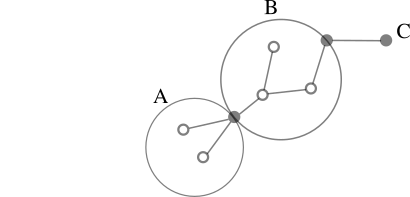
\includegraphics[scale=0.68]{02_dynamic_systems_and_control/png/network_schema}
% \caption{Network Schema}
% \label{fig:network_schema}
% \end{figure}
% 
% Figure \ref{fig:network_schema} shows an inter-network with three networks \verb|A|, \verb|B| and
% \verb|C|. The networks are connected with gateways marked as open circles. The endpoints are marked
% as closed circles. Two gateways \verb|AB| and \verb|BC| are external gateways that interface between
% two networks. All other open circles are internal gateways. Internal gateways are only required to
% understand properties of their own network and also IP. External gateways are only required to
% understand the properties of the two networks they interface with and also IP. There are no
% requirement that gateways understand TCP or any higher-level protocols. The result is that all
% responsibility for TCP is passed to the endpoints.
% 
% This architecture gives a great deal of flexibility, because on the condition that a network
% understands IP the characteristics of its internal network are isolated from the rest of the
% network. It also makes plugging the new network into the inter-network much less complex.
% 
% The problem with this design is that it imposes strong constraints of the network as a feedback
% control system.
% 
% Components in the system have to satisfy network level requirements, but the system was designed to
% strictly minimize the requirements of the gateways.

% TODO: There was a lot of discussion about what 'endpoint' meant.
% TODO: It would have been possible to add congestion information transmission to the gateways, but
% see Jacobson's story about Postel. Also at the time of design, gateways were an expensive
% component in the system, and it wasn't clear at all that congestion would become a problem. 

% TODO: Common pattern in software engineering. The practical approach. Get the components working,
% and then see later if the system works. Can't see into the future what problems will emerge.

% TODO: The important point is that the system doesn't work without a feedback protocol sitting on
% top of IP. It doesn't need to be TCP. But it needs to be responsible for congestion control. The
% connectionless packet idea (IP) is the component that is required of the gateways to know.

% The question is whether the endpoints need extra requirements in IP to send information to the TCP
% level, so as to handle system requirements.

% TODO: But from the point of view of system design, it
% should have been clear that there was a
% problem, to ignore system requirements.

% TODO: This should go earlier in the Cyclades section. 

% This system is feed-forward. The protocol has no mechanism for the sending endpoint to learn
% anything about the receiving protocol. But the network is a limited resource. Each link requires
% time to transmit packets, and each gateway requires time to transmit and has a limited buffer for
% storing queued packets waiting to be re-transmitted. 'best-effort' means that the sending end-point,
% by using the IP protocol, can learn nothing about whether the receiving end-point received the
% message, or the condition of the links and gateways on the route that was used. 
% 
% The TCP protocol is designed as a communication protocol between endpoints. Due to the requirement
% to hide networks, it was designed to work by communication with its other endpoint, called its peer.
% 
% To satisfy the network, i.e. to share out its use fairly and to prevent congestion, the sending peer
% is required to get its feedback response only from information received by the
% 
% This limits the amount of information that

% TODO sharing schema

% TODO layering schema


% chapter:          Dynamic Systems
% section:          Internet
% subsection:       TCP/IP
% subsubsection:    Control System Components
% \subsubsection{Control System Components}
% 
% \begin{figure}[H]
% \centering
% \includegraphics[scale=0.28]{01_introduction/png/feedback_schema}
% \caption{Control System Schema}
% \label{fig:feedback_schema}
% \end{figure}

% chapter:          Dynamic Systems
% section:          Internet
% subsection:       Congestion
% \subsection{Congestion}

% chapter:          Dynamic Systems
% section:          Internet
% subsection:       Congestion
% subsubsection:    TCP Feedback schema 
% \subsubsection{TCP Feedback Schema} 

% \begin{quote}
% By means of simulating TCP/IP network operations we are able to examine in detail the causes of
% traffic oscillation in a simple network setting. Our analysis shows that users' control actions
% are highly synchronized by the network congestion signaling and that providing users only a
%     binary network state can lead to repeated oscillations\cite{zhang1990}.
% \end{quote}


% TODO: Check references [Leland94], [Flo94], [Zha90].

% chapter:          Dynamic Systems
% section:          Internet
% subsection:       Congestion
% subsubsection:    The Actual Design
% \subsection{The Actual Design}

% TODO: Place this image in the correct place

% \begin{figure}[H]
% 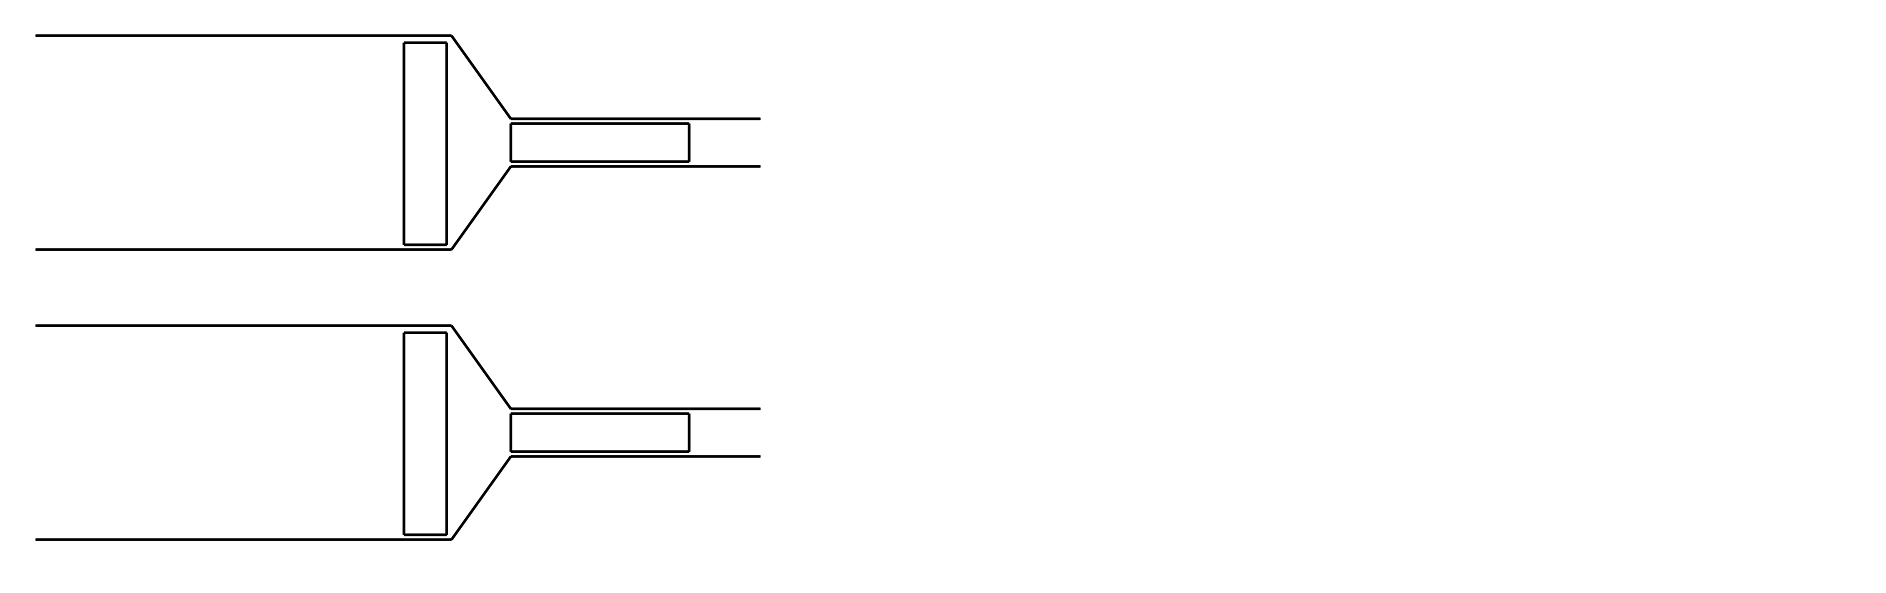
\includegraphics[scale=0.48]{02_dynamic_systems_and_control/png/bandwidth_transition}
% \caption{Packets reaching bandwith transition}
% \label{fig:bandwidth_transition}
% \end{figure}

% ACK clocking is pseudo-mechanical. When this system was designed the cost (monetary and in time)
% of computer processing was large. The IMP (the interface 'card') had 12K of memory and a cost of
% hundreds of thousands of dollars. The ingenuity of mechanical feedback stabilization mechanism is
% remarkable, and given the costs at the time, made sense. In general though, mechanical feedback
% processes are highly inflexible (hence the ingenuity required) compared to a simple PID
% controller.   

% What the actual design looked like

% The problem that occurred

% TODO: Describe the actual events that occurred.

% chapter:          Dynamic Systems
% section:          Internet
% subsection:       Congestion
% subsubsection:    Congestion Events
% \subsubsection{Congestion Events}


% Thinking about the problem as a positive feedback

% chapter:          Dynamic Systems
% section:          Internet
% subsection:       Congestion
% subsubsection:    Positive Feedback 
% \subsubsection{Positive Feedback}


% chapter:          Dynamic Systems
% section:          Internet
% subsection:       Routing
% \subsection{Routing}

% \subsubsection{IP vs TCP}

% From a control system point of view, IP and TCP are separate. IP is fundamentally static. Packets
% are set onto the network, and no measurement or response is taken. TCP is a dynamic process -
% sending packets onto the network, collecting data from the network, and using that data to respond
% to failures.
% 
% European method was IP, US approach was a combination of IP and TCP. In around 1978, the US team
% separated out the (clearly different functionality from a control system point of view) IP and TCP.
% 
% \subsubsection{Dropping Packets}
% 
% Using dropped packets as a error measurement is problematic.
% 
% \subsubsection{Introduction to the Internet}
% 
% Our goal is to examine the different negative and positive feedback systems in the internet. How
% important are these feedbacks to the design of the internet? What are the constraints on the design
% of these feedbacks? Identify which designs have successfully solves problems, and which have not.
% 
% In general feedback design is embedded in algorithms and not so explicit, but are central to network
% design from the beginning. 
% 
% \subsubsection{Cost}
% 
% Telephone networks have serial connections, meaning that failure in any link results in failure of
% the connection. In consequence every link has to be very high reliability and therefore costly.
% Packet switching networks could work across cheap wires and use software design to solve reliability
% problems.
% 
% \subsubsection{Downsides}
% 
% The downsides of packet switching is the requirement for computing power and memory buffers and the
% ends of network links.
% 
% \subsubsection{Social Resistance}
% 
% Roberts\cite{roberts1978} later reflected on the development of packet switching,
% 
% \begin{quote}
% The very fact that no technological breakthrough was required to implement packet switching was
% another factor weighing against its acceptance by the engineering community. What was required was a
% total reevaluation of the performance and economics of dynamic-allocation systems, and their
% application to an entirely different task. Thus, it remained for outsiders to the communications
% industry, computer professionals, to develop packet switching in response to a problem for which the
%     needed a better answer: communicating data to and from computers.
% \end{quote}

% One might expect that the choice of route is determined by feeding back to the routing control
% components in the system, information about round-trip times.
% 
% Very interestingly, this isn't how choice of route is determined.
% 
% In general, route choice is determined statically by the system administrators for each owned
% component of network.  
% 
% This seems surprising on two points,
% 
% \begin{enumerate}
%     \item If route choice is so static how can the system respond to change?
%     \item Routes remain very dynamic. If we use 'traceroute' on an internet request, the route is
%         always changing.
% \end{enumerate}
% 
% The important point is that computer networks are extremely bursty and unpredictable. It is the
% nature of computer network traffic that it occurs in bursts. This introduces large amounts of noise
% into the feedback process. 
% 
% The way to handle this unpredictability is to increase the time-frame response. By aggregating data
% we can smooth out the response. In other words, by making the feedback slower we can increase its
% effectiveness.   
% 
% The companies that own the network are motivated to optimizing the this feedback process. So
% economics comes into the loop.
% 
% One draw-back of economic feedback across the network is that system administrators optimize the
% network for their own customers.
% 
% How does this guarantee that the network is also optimized for temporary non-paying users of that
% network?
% 
% 
% 
% There are a couple of important economic lessons/analogies here:
% 
% 1. aggregating    
% 2. feedback doesn't necessarily have to be built in from the smallest granularity upwards,
%    system-administration of internet areas is sufficient.
% 
% It may well be (though not guaranteed) that the feedback in aggregated systems (such as the whole
% economy) can work well, even if the components are clumpy (as in administrative areas in the
% internet). [reword]
% 
% It is not a-priory guaranteed that such systems are stable or unstable. Ultimately, the stability of
% a system can only be guaranteed through a process of redesign and testing (i.e. a scientific
% process).
% 
% This is also experienced with the internet - we can see that iterative improvement process at all
% levels, and redesign responses to failure.

% [history of fixing the problems of the internet]

